% ==============================================================================
%  技术文档：三维力导向图物理仿真与状态空间可视化系统
%  项目：华容道 (Klotski) 状态空间探索与 3D 可视化
% ==============================================================================
\documentclass[11pt,a4paper]{report}
% ==============================================================================
% --- ctex 中文配置 --------------------------------------------------------------
\usepackage[UTF8, heading=true]{ctex}
% --- 页面布局 ----------------------------------------------------------------
\usepackage[top=3cm,bottom=3cm,left=3cm,right=3cm]{geometry}
\usepackage{setspace}
\onehalfspacing
\usepackage{fancyhdr}
\pagestyle{fancy}
\fancyhf{}
\fancyhead[LE]{\small\nouppercase\leftmark}
\fancyhead[RO]{\small\nouppercase\rightmark}
\fancyfoot[LE,RO]{\thepage}
\renewcommand{\headrulewidth}{0.4pt}
% --- 数学符号 ----------------------------------------------------------------
\usepackage{amsmath,amssymb,amsthm}
\usepackage{mathtools}
\usepackage{bm}
% --- 图形与浮动体 ------------------------------------------------------------
\usepackage{graphicx}
\usepackage{caption}
\usepackage{subcaption}
\usepackage{float}
\usepackage{booktabs}
\usepackage{array}
\usepackage{multirow}
\usepackage[table]{xcolor}
% --- 代码排版 ----------------------------------------------------------------
\usepackage{listings}
\usepackage{xcolor}
\definecolor{codebg}{rgb}{0.95,0.95,0.97}
\definecolor{codeframe}{rgb}{0.80,0.80,0.85}
\definecolor{codekey}{rgb}{0.12,0.29,0.53}
\definecolor{codestr}{rgb}{0.60,0.20,0.20}
\definecolor{codecom}{rgb}{0.35,0.55,0.35}
\lstdefinestyle{pythonstyle}{
    language=Python,
    backgroundcolor=\color{codebg},
    basicstyle=\small\ttfamily,
    keywordstyle=\color{codekey}\bfseries,
    stringstyle=\color{codestr},
    commentstyle=\color{codecom}\itshape,
    numberstyle=\tiny\ttfamily,
    numbers=left,
    numbersep=6pt,
    frame=single,
    rulecolor=\color{codeframe},
    breaklines=true,
    tabsize=4,
    captionpos=b,
    showstringspaces=false,
    literate={_}{\_}1,
    morekeywords={ti,glm,glfw,gl,GL,glUniformMatrix4fv,glBindBuffer,
                  glGenVertexArrays,glGenBuffers,glVertexAttribPointer,
                  glEnableVertexAttribArray,glDrawArrays,
                  compileShader,compileProgram,glm},
}
\lstnewenvironment{pythoncode}{\lstset{style=pythonstyle}}{}
% --- 超链接与引用 ------------------------------------------------------------
\usepackage[colorlinks=true,linkcolor=blue!60!black,citecolor=blue!60!black,
            urlcolor=blue!60!black]{hyperref}
\usepackage{cleveref}
% --- 定理与定义环境 ----------------------------------------------------------
\newtheorem{definition}{定义}[chapter]
\newtheorem{theorem}{定理}[chapter]
\newtheorem{lemma}{引理}[chapter]
\newtheorem{corollary}{推论}[chapter]
% --- 标题页 ------------------------------------------------------------------
\title{\vspace{-2cm}
       \textbf{三维力导向图物理仿真 \\[0.3em]
              与状态空间可视化系统} \\[0.6em]
       \large 基于 GPU 加速的华容道滑块谜题 \\[0.2em]
       状态空间探索与可视化平台}
\author{技术文档}
\date{\today}
\begin{document}
\maketitle
% --- 摘要 --------------------------------------------------------------------
\begin{abstract}
本文档描述了一套用于探索滑块谜题状态空间的三维力导向图可视化系统的设计、
数学基础与实现。系统以经典华容道（Klotski）谜题为主要应用对象，包含四个
核心模块：(i)~滑块谜题引擎，支持任意矩形棋盘的建模与全状态空间广度优先
枚举；(ii)~基于 \texttt{Taichi} 框架的 GPU 加速物理仿真引擎，在数千节点
规模上并行计算库仑式斥力与弹簧式引力；(iii)~基于 OpenGL~3.3~Core~Profile
的自定义三维渲染器，提供实时交互与自动相机控制；(iv)~异步视频录制管道，
将图结构的生长过程与后续环绕观察导出为高质量 MPEG-4 视频。本文详述了
力模型的数学推导、基于广度优先搜索（BFS）的图构建算法、基于着色器的深度
衰减渲染管线，以及十六种华容道谜题配置及其状态空间统计。
\end{abstract}
% --- 目录 --------------------------------------------------------------------
\tableofcontents
\listoffigures
\listoftables
% ==============================================================================
\chapter{引言}
\label{ch:introduction}
% ==============================================================================
\section{研究动机}
\label{sec:motivation}
滑块谜题（sliding-block puzzle），如华容道（Klotski），是一类经典的组合
谜题：若干矩形木块须在有限的棋盘区域内移动，以使得指定木块到达目标出口。
尽管规则简单，此类谜题的表达能力却令人惊讶——某些配置属于
PSPACE-完全类问题~\cite{hearn2006slides}，意味着在最坏情况下，求解最短
路径的复杂度随问题规模呈指数增长。
对于典型的含十个以上木块的华容道，不同的棋盘布局（即\textbf{状态空间}）
可达数万种。每个状态对应图中的一个节点，每步合法移动对应一条边。理解该
图的全局结构——其直径、分支因子、聚类系数以及解路径的几何排布——对于
求解算法的设计者与希望欣赏谜题景观的爱好者都具有重要价值。
然而，原始的邻接矩阵或二维弹簧布局在节点数超过数百时即变得难以解读。

本项目受 twoswap 的力导向图动画~\cite{twoswap2024} 启发，将类似的可视化
方法推广至滑块谜题的状态空间分析。项目的完整源代码已开源发布于
GitHub~\cite{klotski-github}，作者制作的演示视频可在
Bilibili~\cite{klotski-bilibili} 与 YouTube~\cite{klotski-youtube}
上观看。

这促使我们构建一个三维力导向可视化系统，以实现以下目标：
\begin{enumerate}
    \item 自动枚举给定谜题的完整状态空间；
    \item 通过精心调校的力导向模型在三维空间中布局生成的图，使聚类与桥接
          结构在视觉上清晰可辨；
    \item 以广度优先遍历方式从起始状态开始逐节点\emph{生长}图结构，并
          制作动画；
    \item 实时渲染场景，支持三维交互控制，并将动画导出为视频文件。
\end{enumerate}
\section{系统概览}
\label{sec:overview}
图~\ref{fig:system-architecture} 展示了系统的高层架构。五个 Python 模块
以流水线方式协作：
\begin{description}
    \item[\texttt{Klotski.py}] 建模滑块谜题棋盘，枚举合法移动，构建全局
        状态空间图。
    \item[\texttt{GraphHelper.py}] 在图表示形式（邻接矩阵、边列表、邻接表）
        之间进行转换。
    \item[\texttt{GraphPhysics.py}] 核心物理引擎，通过 \texttt{Taichi}
        内核加速库仑斥力计算。维护一个 BFS 驱动的生长模拟，逐步揭示节点。
    \item[\texttt{GraphRender.py}] 基于 OpenGL~3.3 的自定义渲染器，提供
        GLSL 着色器、相机控制与自动距离调整。
    \item[\texttt{VideoRecorder.py}] 异步帧捕获与编码器，叠加进度信息并
        写入 MPEG-4 视频。
\end{description}
\begin{figure}[htbp]
    \centering
    \fbox{\parbox{0.85\textwidth}{\centering
    \vspace{1.5cm}
    \textbf{流水线结构} \\[0.5cm]
    $\texttt{Klotski.py} \;\rightarrow\; \texttt{GraphHelper.py}
      \;\rightarrow\; \texttt{GraphPhysics.py}
      \;\rightarrow\; \texttt{GraphRender.py}
      \;\rightarrow\; \texttt{VideoRecorder.py}$ \\[0.3cm]
    \small （箭头方向表示数据流）\\[1.5cm]
    }}
    \caption{系统架构与数据流。谜题状态空间经枚举后被转换为邻接结构，
             送入力导向物理仿真，经 OpenGL 进行三维渲染，并可选地录制
             为视频文件。}
    \label{fig:system-architecture}
\end{figure}
主入口点为 \texttt{PlayGround.py}，它实例化选定的谜题配置，构建图，
创建物理仿真，并启动交互式查看器或批量视频导出模式。
\section{相关工作}
\label{sec:related}
力导向图布局可追溯至 Eades~\cite{eades1984heuristic} 与
Fruchterman--Reingold~\cite{fruchterman1991graph} 的开创性工作，至今仍是
网络可视化的基石。本文使用的弹簧--电荷模型是 \texttt{Graphviz}~\cite{ellson2001graphviz}
和 \texttt{networkx} 等流行工具所采用方法的变体。近期研究已将这些技术
扩展到三维布局并通过 GPU 加速~\cite{liu2014gpu}，本系统通过
\texttt{Taichi} 框架~\cite{hu2019taichi} 采纳了这一方向。
滑块谜题的状态空间分析在十五数码问题及其推广中已有研究~\cite{ratner1986finding}。
华容道谜题尤其受到多位学者~\cite{hearn2006slides} 的关注，其 PSPACE-完全
性已被证明。据我们所知，本系统是首个将完整状态空间枚举、GPU 加速三维
力导向布局与视频导出集成于单一工具中的滑块谜题可视化平台。
% ==============================================================================
\chapter{滑块谜题基础}
\label{ch:puzzle}
% ==============================================================================
\section{问题定义}
\label{sec:problem-def}
滑块谜题由一个 $W \times H$（宽~$\times$~高）的矩形棋盘和 $B$ 个矩形
木块定义。每个木块 $b_i$ ($i = 0, \ldots, B-1$) 的大小为
$(w_i, h_i)$，在棋盘上占据位置 $(x_i, y_i)$，其中 $x_i, y_i$ 为非负整数，
且满足 $0 \le x_i < W$、$0 \le y_i < H$。一个配置\emph{合法}当且仅当：
\begin{enumerate}
    \item 任意两木块不重叠：对任意 $i \neq j$，矩形区域
          $[x_i, x_i + w_i) \times [y_i, y_i + h_i)$ 与
          $[x_j, x_j + w_j) \times [y_j, y_j + h_j)$ 不相交。
    \item 每块木块完全位于棋盘内：对所有 $i$ 有
          $x_i + w_i \le W$ 且 $y_i + h_i \le H$。
\end{enumerate}
\textbf{合法移动}指将单个木块沿上、下、左、右四个基本方向之一平移一个
单位，且平移后的配置保持合法。\textbf{状态空间}是从给定起始配置出发，
通过合法移动序列可达的所有配置的集合，连同连接它们的移动本身。
\begin{definition}[状态空间图]
设 $\mathcal{C}$ 为给定谜题的所有合法配置的集合。状态空间图是无向图
$G = (V, E)$，其中 $V = \mathcal{C}$，且 $(u, v) \in E$ 当且仅当存在
一个合法移动将配置 $u$ 变换为配置 $v$。
\end{definition}
\section{华容道谜题}
\label{sec:klotski}
经典华容道（图~\ref{fig:klotski-layout}）使用 $4 \times 5$ 棋盘与
10 块木块：
\begin{itemize}
    \item \textbf{1} 块 $2\times2$ 大方块（曹操）——必须到达底部的出口。
    \item \textbf{5} 块 $1\times2$ 竖方块（关羽、张飞、赵云、马超、黄忠）。
    \item \textbf{4} 块 $1\times1$ 小方块（兵卒）。
\end{itemize}
\begin{figure}[htbp]
    \centering
    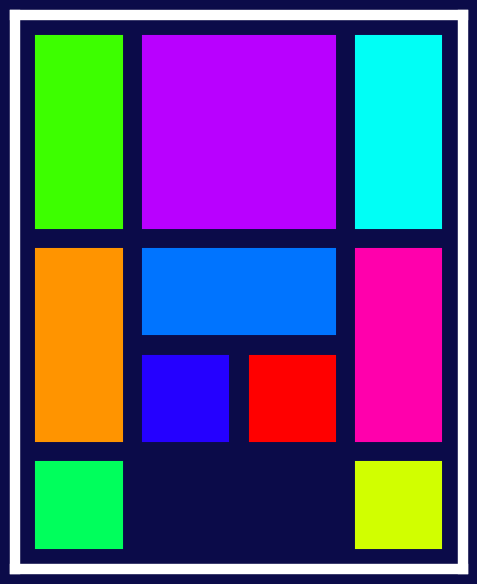
\includegraphics[width=0.35\textwidth]{Figure1.png}
    \caption{经典 $4\times5$ 华容道初始布局。中央为 $2\times2$ 的曹操；
             五块 $1\times2$ 竖块分列两侧；四块 $1\times1$ 兵卒占据
             底部一行。}
    \label{fig:klotski-layout}
\end{figure}
\section{棋盘表示}
\label{sec:representation}
系统内部将每个配置存储为两个整数数组：
\begin{itemize}
    \item \texttt{box\_sizes} —— 形状 $(B, 2)$，存储各木块的
          $(w_i, h_i)$。
    \item \texttt{box\_positions} —— 形状 $(B, 2)$，存储各木块的
          $(x_i, y_i)$。
\end{itemize}
辅助函数 \texttt{get\_covering\_matrix} 将所有木块栅格化到一张
$H \times W$ 的占用网格上：
\begin{equation}
    M_{rc} = \sum_{i=0}^{B-1} \mathbf{1}\big[x_i \le c < x_i + w_i \;\land\;
              y_i \le r < y_i + h_i\big]
\end{equation}
一个配置合法当且仅当对所有 $(r,c)$ 有 $M_{rc} \le 1$，且无木块超出
棋盘边界。
\subsection{状态标识}
\label{sec:state-id}
为高效检测两配置是否相同（BFS 期间的必需操作），我们计算一个\emph{标识
矩阵}，该矩阵对木块的标签不敏感。对每个格子 $(r,c)$，其标识值为：
\begin{equation}
    I_{rc} = \sum_{i} \mathbf{1}[\text{木块 } i \text{ 覆盖 } (r,c)]
             \cdot (2^{w_i} \cdot 3^{h_i})
\end{equation}
此方案为每种尺寸的木块分配一个独特的质数乘积指纹，使得各行构成的元组
$(I_{r0}, \ldots, I_{r,W-1})$ 可作为规范哈希。两配置相等当且仅当它们的
标识矩阵逐元素相同。
\subsection{邻居枚举}
\label{sec:neighbour}
对每块木块 $i$，我们考察四个候选平移方向
$\Delta \in \{ \text{上}, \text{下}, \text{左}, \text{右} \}$，
对应沿各轴的单位位移。一个候选移动合法当且仅当：
\begin{enumerate}
    \item 平移后的木块不超出棋盘边界。
    \item 木块移入和移出的格子不会导致任何格子出现 $M_{rc} > 1$。
\end{enumerate}
由于覆盖矩阵始终可用且每次查询为 $\mathcal{O}(1)$，每个邻居检查对大小为
$(w_i, h_i)$ 的木块耗时 $\mathcal{O}(w_i + h_i)$，因为我们只需检查运动
方向上的那些格子。
\subsection{有墙变体}
\label{sec:walled}
\texttt{WalledSlidingToy} 子类施加了额外的约束：木块只能在其尺寸为~1 的
轴向上移动（即 $1\times2$ 的木块仅可竖直滑动，$2\times1$ 的木块仅可
水平滑动）。此限制模拟了某些物理谜题中由榫接或滑槽限制自由度的情形。
% ==============================================================================
\chapter{状态空间枚举}
\label{ch:enumeration}
% ==============================================================================
\section{广度优先搜索}
\label{sec:bfs}
完整状态空间通过标准广度优先搜索进行枚举，如算法~\ref{alg:bfs} 所示。
\begin{figure}[htbp]
\begin{lstlisting}[style=pythonstyle,numbers=none,
    caption={构建全局状态空间图},
    label=alg:bfs]
输入:  start_toy  (初始 SlidingToy 配置)
       maxiter    (可选的最大 BFS 迭代次数)
输出: adj        (稀疏邻接矩阵, scipy.sparse.csr)
       state2idx (字典: 状态哈希 -> 整数索引)
       idx2state (列表: 索引 -> SlidingToy 实例)
       edges     ((u, v) 无向边元组列表)
state2idx[start] := 0
idx2state[0] := start_toy
current_visitors := [start_toy]
while current_visitors 非空 AND 迭代次数 < maxiter:
    next_visitors := []
    for each 状态 in current_visitors:
        cur_idx := state2idx[hash(状态)]
        for each 邻居 n of 状态:
            if hash(n) not in state2idx:
                state2idx[hash(n)] := |state2idx|
                idx2state.append(n)
                next_visitors.append(n)
            neigh_idx := state2idx[hash(n)]
            if cur_idx < neigh_idx:       # 避免重复边
                edges.append((cur_idx, neigh_idx))
    current_visitors := next_visitors
\end{lstlisting}
\end{figure}
算法逐层推进，为最新发现的状态分配整数索引。边仅记录一次
（条件 \lstinline{cur_idx < neigh_idx} 在无向图中保证了这一点）。
最终的邻接矩阵以稀疏 \texttt{COO} 格式构建：
\begin{equation}
    A_{ij} = \begin{cases}
        1 & \text{若 } (i,j) \in E, \\
        0 & \text{否则}.
    \end{cases}
\end{equation}
\subsection{复杂度分析}
\label{sec:complexity}
设 $N = |V|$ 为不同状态数，$E = |E|$ 为边数。每个状态至多生成 $4B$ 个
候选邻居（因为 $B$ 块木块每块至多可向四个方向移动）。哈希查找
\lstinline{hash(n) in state2idx} 的摊还成本为 $\mathcal{O}(1)$。
因此总时间复杂度为：
\begin{equation}
    \mathcal{O}(N \cdot B \cdot (w_{\max} + h_{\max}) + E)
\end{equation}
其中 $w_{\max}$ 与 $h_{\max}$ 为影响重叠检查开销的最大木块尺寸。
实践中，对于 $N \approx 20\,000$、$B = 10$ 的经典华容道，枚举在主流
台式 CPU 上可在两秒内完成。

\begin{figure}[htbp]
    \centering
    \begin{subfigure}[b]{0.47\textwidth}
        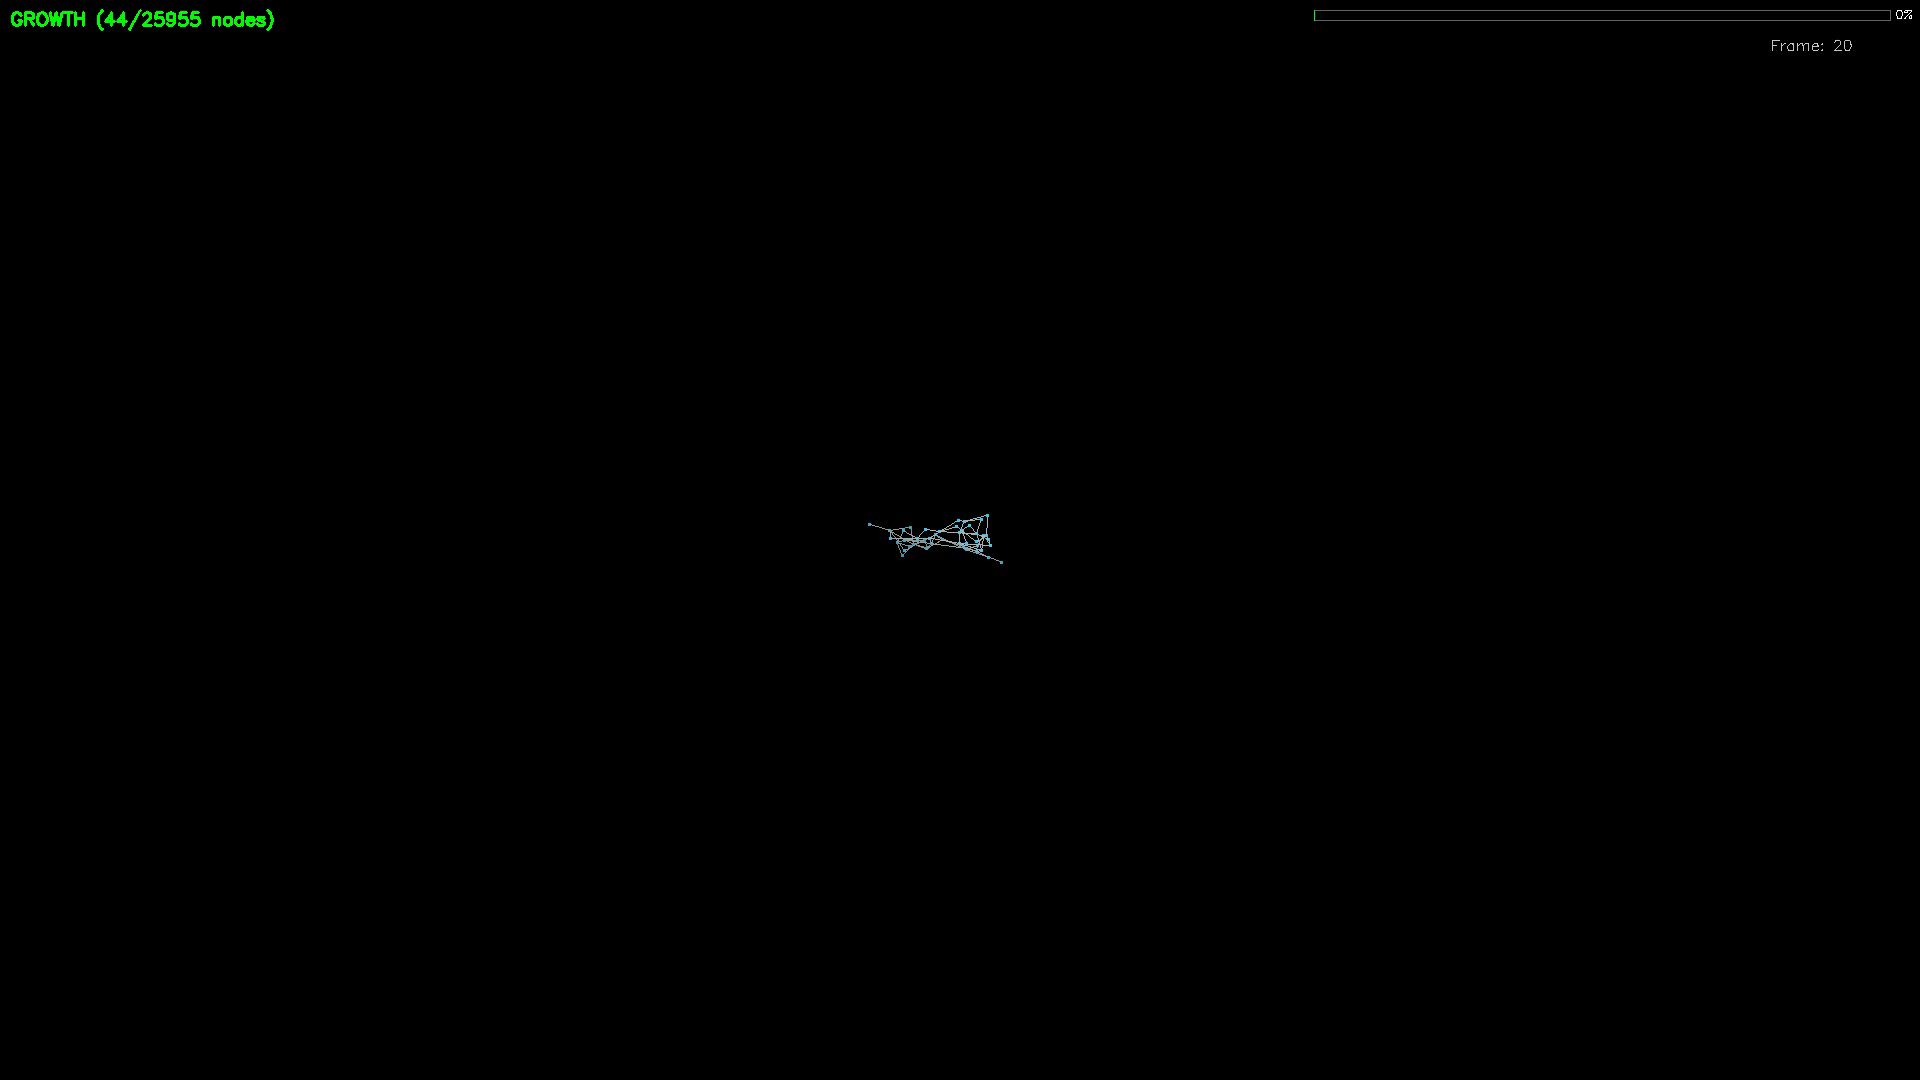
\includegraphics[width=\textwidth]{screenshot_01.png}
        \caption{生长初期，BFS 刚展开数十个节点，图结构稀疏。}
        \label{fig:growth-01}
    \end{subfigure}
    \hfill
    \begin{subfigure}[b]{0.47\textwidth}
        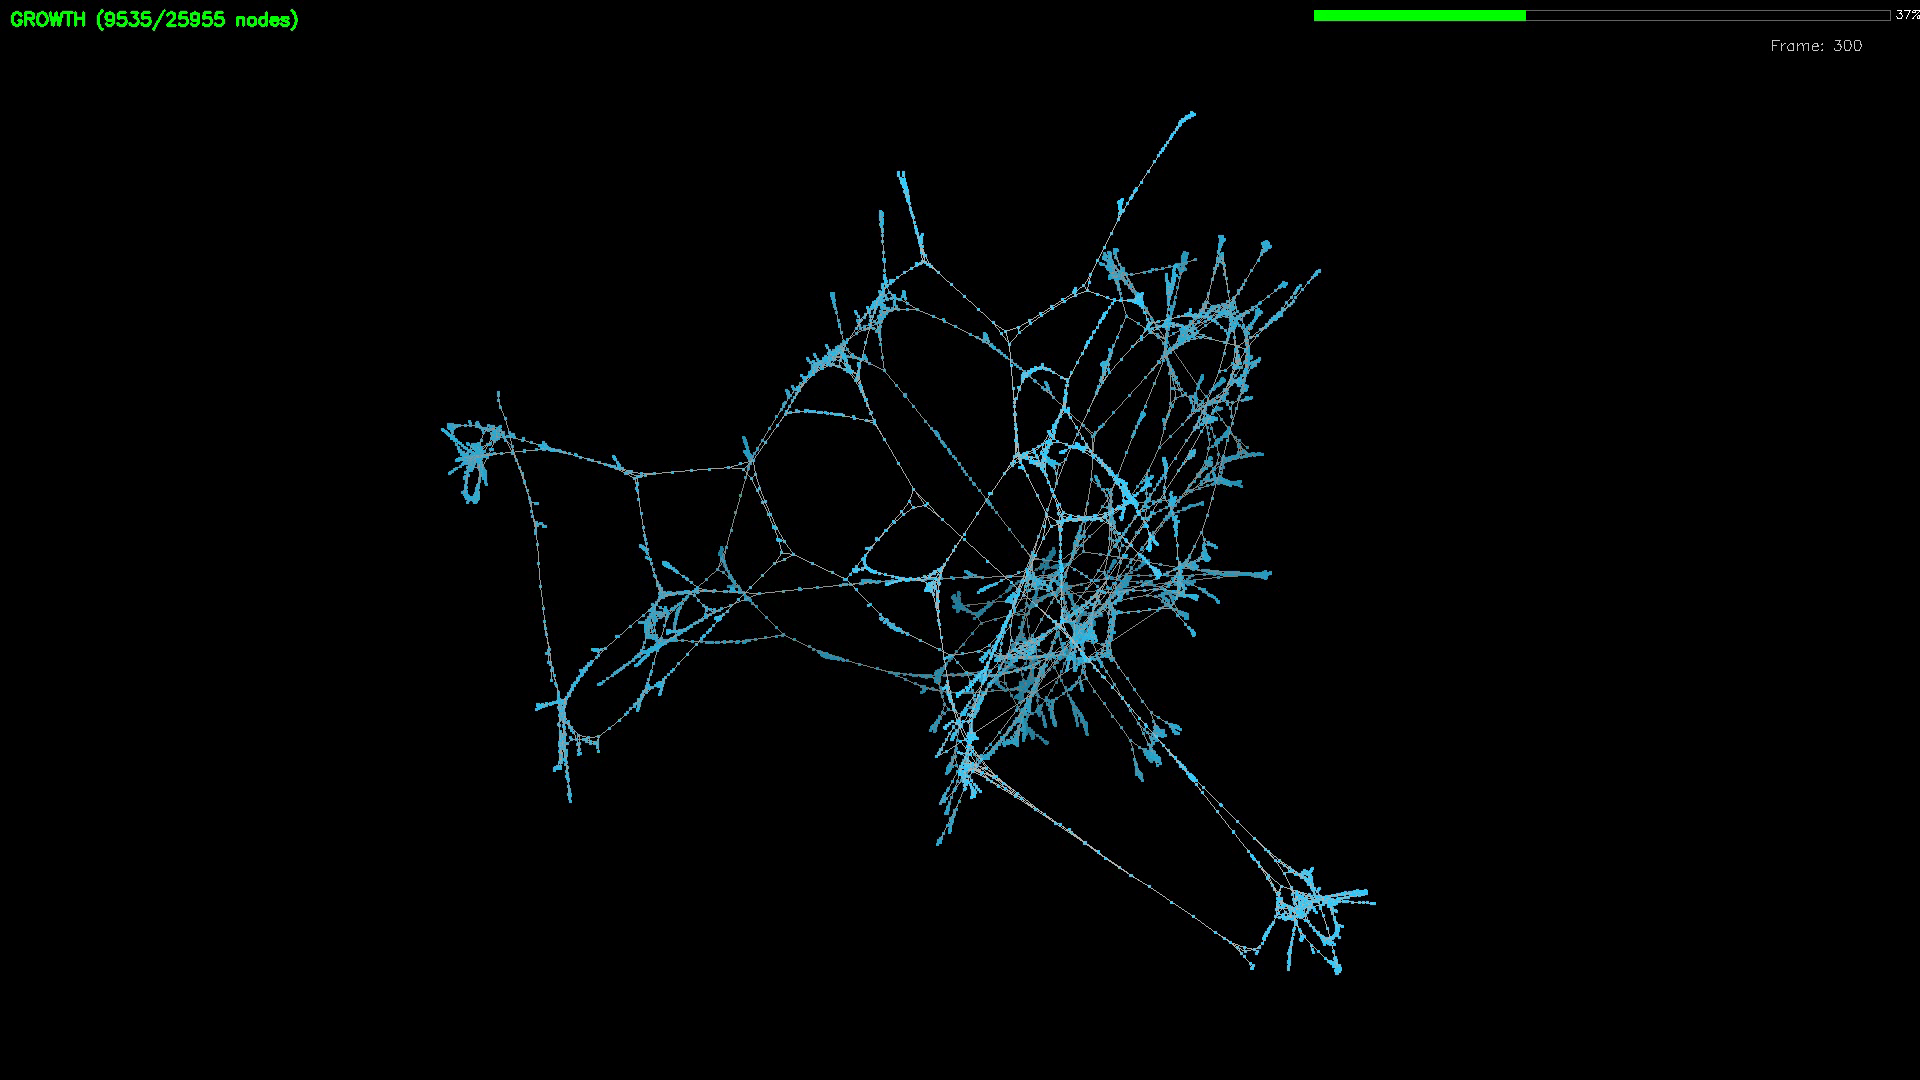
\includegraphics[width=\textwidth]{screenshot_02.png}
        \caption{生长约 1/3 处，节点快速增加，核心聚类开始形成。}
        \label{fig:growth-02}
    \end{subfigure}
    \vskip\baselineskip
    \begin{subfigure}[b]{0.47\textwidth}
        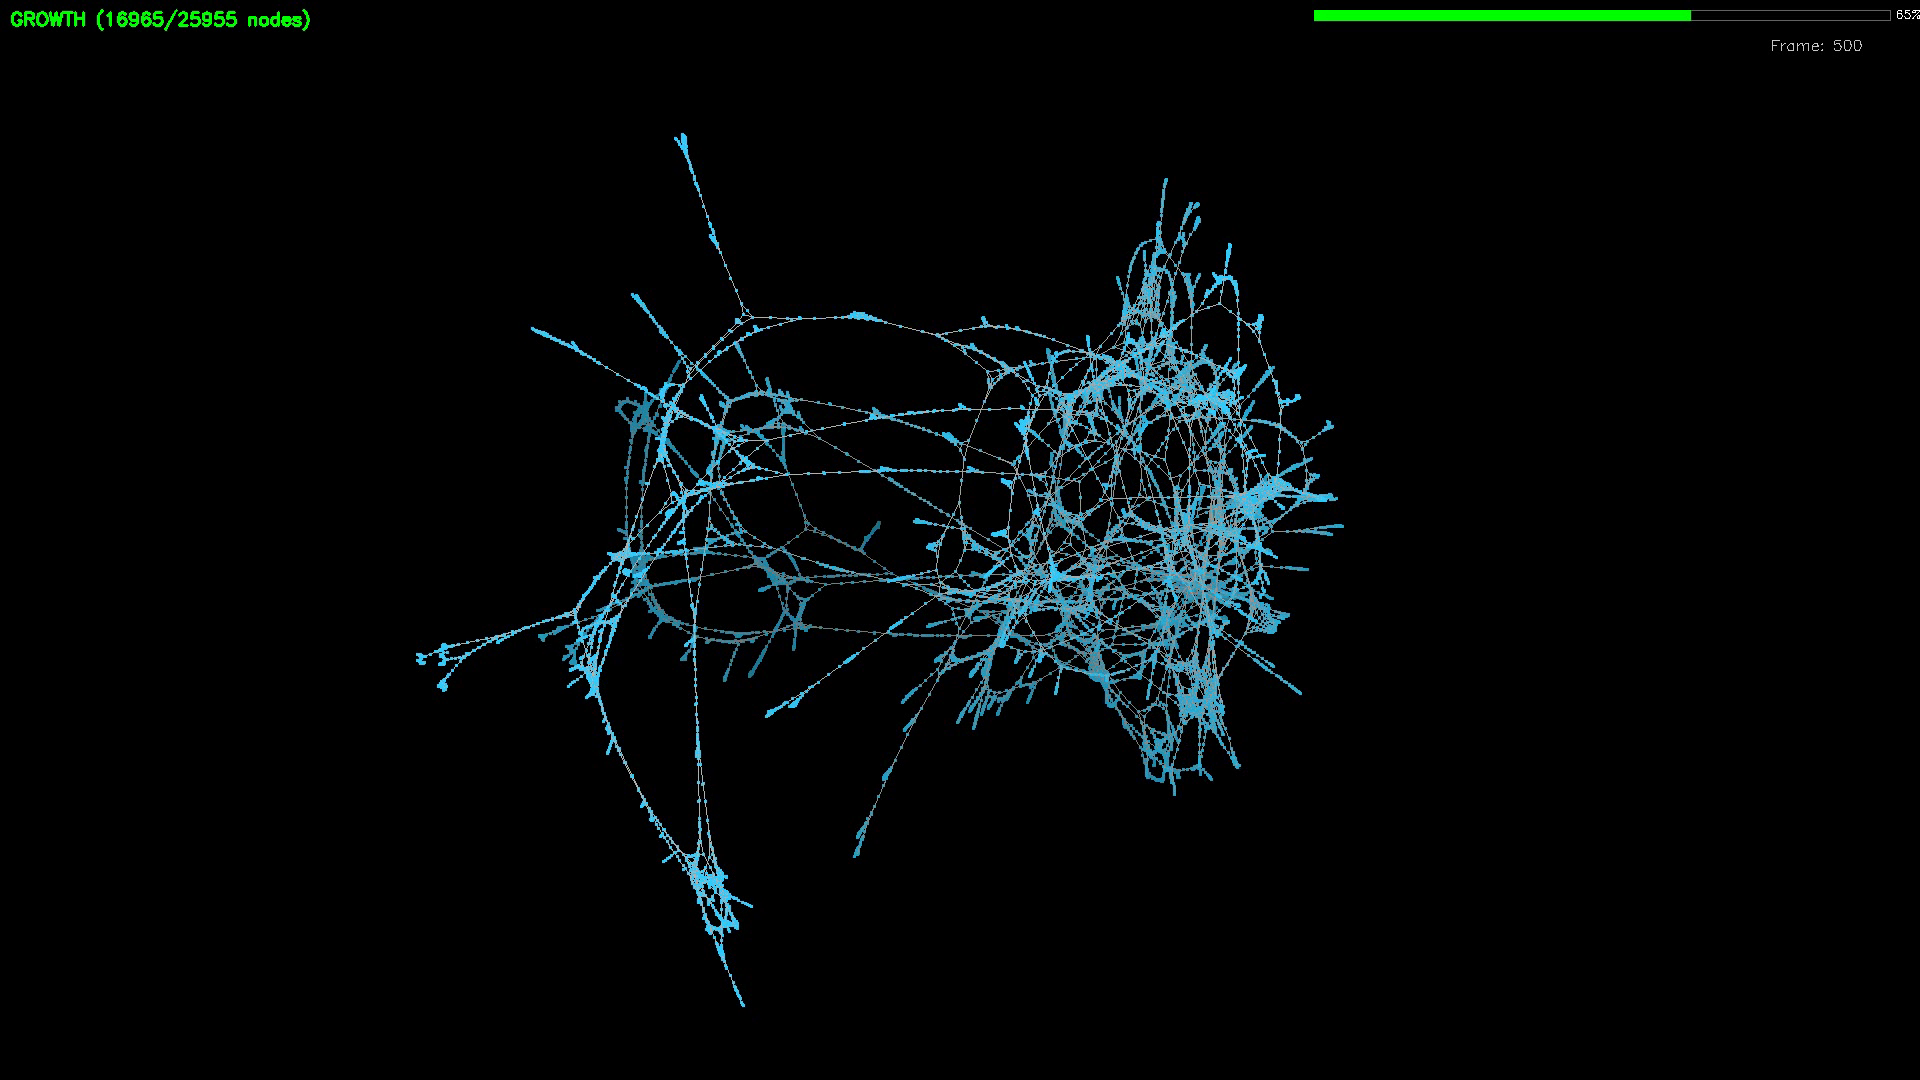
\includegraphics[width=\textwidth]{screenshot_03.png}
        \caption{生长约 2/3 处，大部分节点已激活，图结构逐渐收敛。}
        \label{fig:growth-03}
    \end{subfigure}
    \hfill
    \begin{subfigure}[b]{0.47\textwidth}
        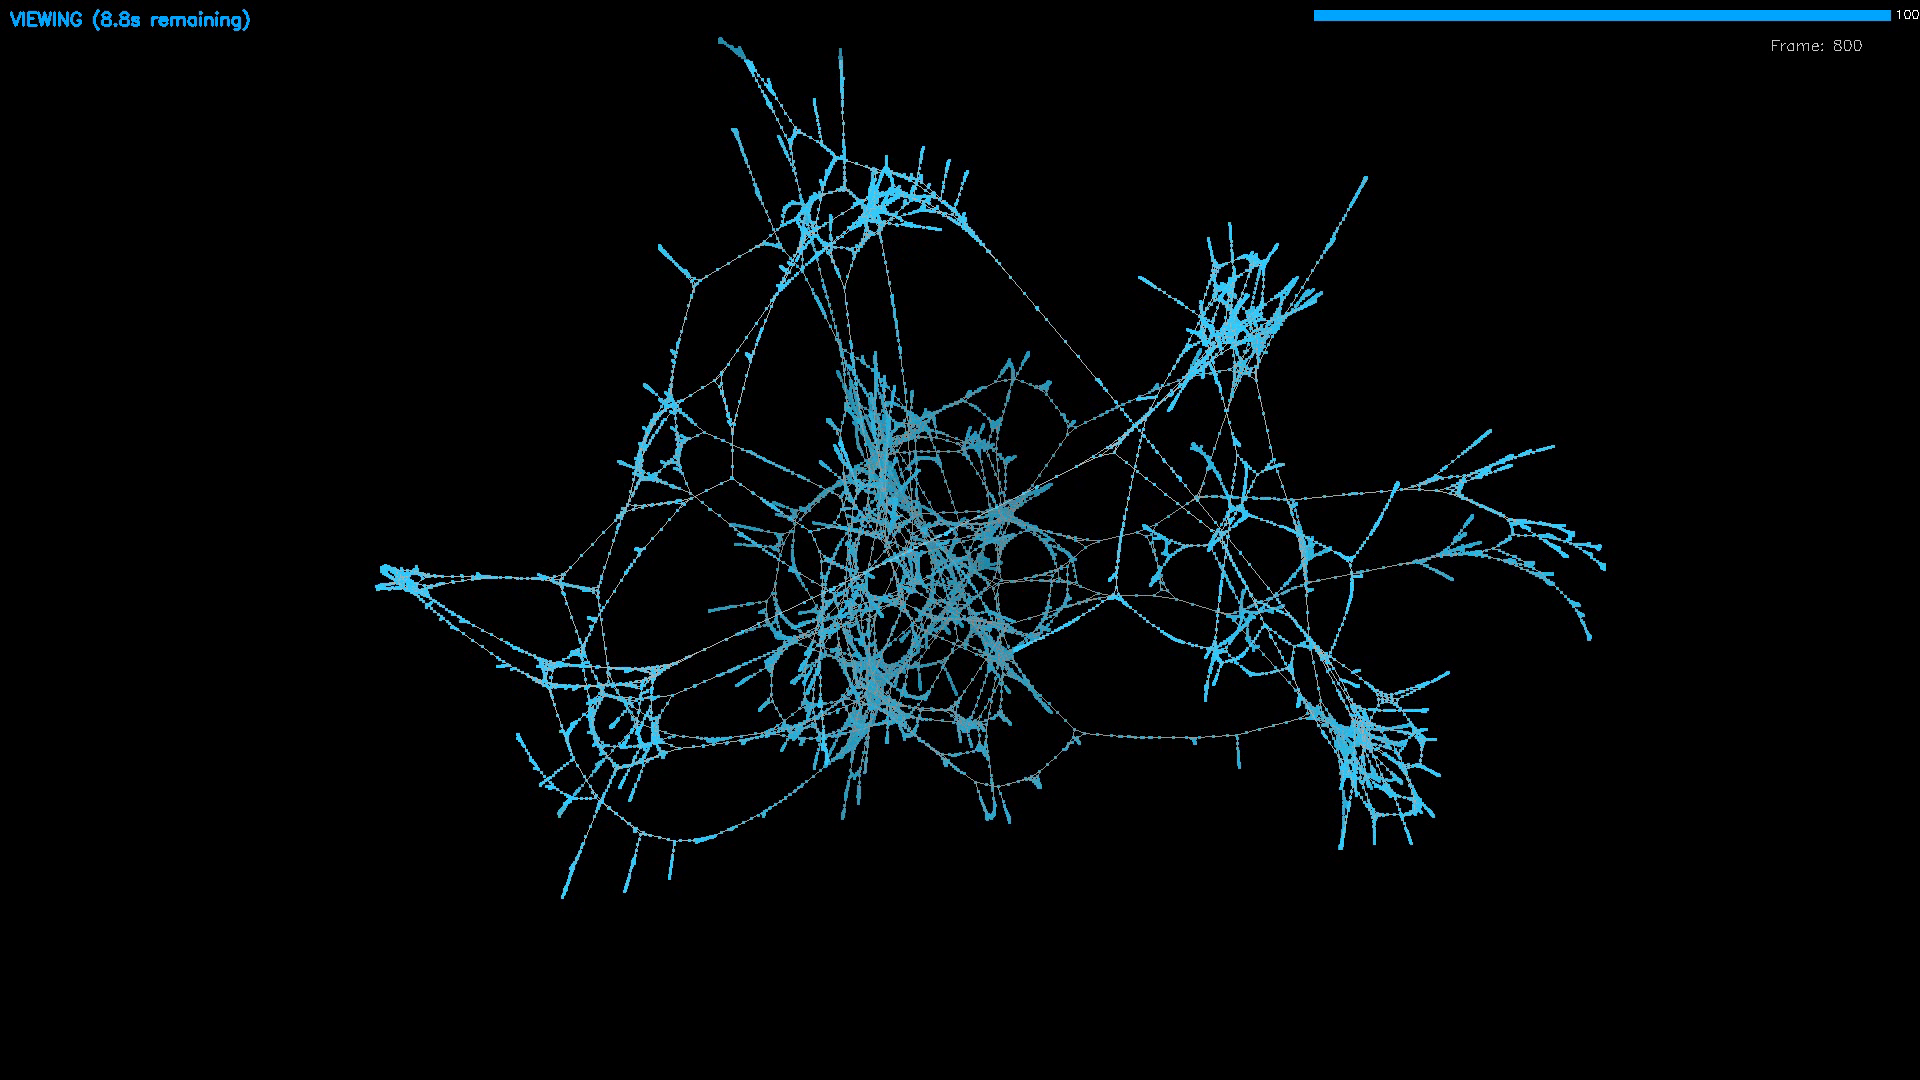
\includegraphics[width=\textwidth]{screenshot_04.png}
        \caption{生长完成，所有 $\sim$20\,000 个节点已布局，进入环绕观赏阶段。}
        \label{fig:growth-04}
    \end{subfigure}
    \caption{华容道（谜题~1）状态空间图从根节点出发逐层生长的四个阶段，
             截图等间距取自自动渲染视频。完整生长与观赏动画见
             Bilibili~\cite{klotski-bilibili} 与
             YouTube~\cite{klotski-youtube}。}
    \label{fig:growth-sequence}
\end{figure}

\section{图的表示}
\label{sec:graph-repr}
枚举得到的图以三种可互换的形式表示：
\begin{itemize}
    \item \textbf{边列表} —— $\mathcal{O}(E)$ 存储，方便构建与序列化。
    \item \textbf{邻接矩阵}（稀疏 CSR）—— $\mathcal{O}(N + E)$ 存储，
          被 \texttt{networkx} 所需，且对矩阵运算高效。
    \item \textbf{邻接表}（字典的列表）—— $\mathcal{O}(N + E)$ 存储，
          物理仿真使用此形式进行邻居迭代。
\end{itemize}
三者之间的转换由 \texttt{GraphHelper.py} 中的
\texttt{edges\_to\_adjacency\_list()} 与
\texttt{matrix\_to\_adjacency\_list()} 完成。
\section{示例谜题的状态空间统计}
\label{sec:puzzle-stats}
表~\ref{tab:puzzles} 列出了本系统包含的十六种谜题配置。每种配置均经过
穷举枚举（在可行范围内）以获得状态计数。
\begin{table}[htbp]
\centering
\caption{华容道谜题配置及其状态空间规模}
\label{tab:puzzles}
\begin{tabular}{crrcl}
\toprule
\textbf{编号} & \textbf{棋盘} & \textbf{木块数} & \textbf{变体} & \textbf{状态数 ($N$)} \\
\midrule
1  & $4 \times 5$ & 10 & 经典 & $\sim$20\,000 \\
2  & $6 \times 6$ & 13 & 有墙 & \\
3  & $4 \times 4$ & 3  & 经典 & $\sim$300 \\
4  & $4 \times 5$ & 7  & 经典 & \\
5  & $4 \times 5$ & 6  & 经典 & \\
6  & $4 \times 6$ & 11 & 经典 & \\
7  & $4 \times 6$ & 7  & 经典 & \\
8  & $4 \times 5$ & 15 & 经典 & \\
9  & $4 \times 5$ & 14 & 经典 & \\
10 & $6 \times 6$ & 10 & 有墙 & \\
11 & $6 \times 6$ & 6  & 有墙 & \\
12 & $4 \times 5$ & 9  & 经典 & \\
13 & $5 \times 5$ & 7  & 经典 & \\
14 & $6 \times 6$ & 13 & 有墙 & \\
15 & $6 \times 6$ & 8  & 有墙 & \\
16 & $6 \times 6$ & 13 & 有墙 & \\
\bottomrule
\end{tabular}
\end{table}
% ==============================================================================
\chapter{力导向图物理仿真}
\label{ch:physics}
% ==============================================================================
\section{力模型}
\label{sec:force-model}
布局通过力导向模型计算，该模型在连续时间 $t$ 上演化节点位置
$\mathbf{p}_i(t) \in \mathbb{R}^3$。每个节点受到三类力的作用。
\subsection{库仑斥力}
\label{sec:repulsion}
任意两个不同节点 $(i, j)$ 之间施加类库仑斥力：
\begin{equation}
    \mathbf{f}^{\text{rep}}_{i \leftarrow j} =
    \frac{k_{\text{coul}}^2}{\|\mathbf{p}_i - \mathbf{p}_j\|^2 + \varepsilon}
    \cdot (\mathbf{p}_i - \mathbf{p}_j)
    \label{eq:coulomb}
\end{equation}
其中 $k_{\text{coul}}$ 为用户可调常数（默认~25），$\varepsilon = 10^{-4}$
为软化参数，防止节点重合时出现奇点。注意到该表达式中 $(\mathbf{p}_i -
\mathbf{p}_j)$ 的模长为 $r = \|\mathbf{p}_i - \mathbf{p}_j\|$，因此
斥力\textbf{大小}为：
\begin{equation}
    \|\mathbf{f}^{\text{rep}}_{i \leftarrow j}\|
    = \frac{k_{\text{coul}}^2}{r^2 + \varepsilon} \cdot r
    \approx \frac{k_{\text{coul}}^2}{r}
    \label{eq:coulomb-mag}
\end{equation}
这是一个 $1/r$ 型的力律，与二维空间中点电荷的电场强度类似。节点 $i$ 上
的总斥力为：
\begin{equation}
    \mathbf{f}^{\text{rep}}_i = \sum_{j \neq i} \mathbf{f}^{\text{rep}}_{i \leftarrow j}
    \label{eq:rep-total}
\end{equation}
\subsection{胡克引力（弹簧模型）}
\label{sec:attraction}
边对连接的节点施加弹簧式引力。对每条边 $(u, v)$：
\begin{equation}
    \mathbf{f}^{\text{att}}_{u \leftarrow v} =
    -\frac{\|\mathbf{p}_u - \mathbf{p}_v\|}{k_{\text{coul}}}
    \cdot (\mathbf{p}_u - \mathbf{p}_v)
    \label{eq:hooke}
\end{equation}
该力的大小随分离距离平方增长：
\begin{equation}
    \|\mathbf{f}^{\text{att}}_{u \leftarrow v}\|
    = \frac{r}{k_{\text{coul}}} \cdot r
    = \frac{r^2}{k_{\text{coul}}}
    \label{eq:hooke-mag}
\end{equation}
即引力大小正比于 $r^2$（二次弹簧），弹簧常数为 $1/k_{\text{coul}}$。
这一反直觉的设计（斥力 $1/r$ 而引力 $r^2$）确保连接节点间的平衡距离
可控且与 $k_{\text{coul}}$ 直接相关，详见第~\ref{sec:force-balance} 节。
\subsection{中心引力}
\label{sec:gravity}
一个弱谐波回复力将所有节点拉向原点：
\begin{equation}
    \mathbf{f}^{\text{grav}}_i = -k_{\text{grav}} \cdot \mathbf{p}_i
    \label{eq:gravity}
\end{equation}
默认 $k_{\text{grav}} = 0.02$。此力防止图结构在斥力作用下无限漂移。
\subsection{阻尼}
\label{sec:damping}
速度比例阻尼确保系统收敛至稳定平衡而非持续振荡：
\begin{equation}
    \mathbf{v}_i^{(t+1)} = \beta \left( \mathbf{v}_i^{(t)} +
        \frac{\mathbf{f}_i}{m_i} \Delta t \right),
    \qquad \mathbf{p}_i^{(t+1)} = \mathbf{p}_i^{(t)} +
        \mathbf{v}_i^{(t+1)} \Delta t
    \label{eq:damping}
\end{equation}
阻尼系数 $\beta = 0.8$，时间步 $\Delta t = 0.15$，所有节点单位质量
（$m_i = 1$）。速度限幅 $\|\mathbf{v}_i\|_{\max} = 10$ 可防止布局初期
力较大时出现数值不稳定。
\subsection{力平衡分析}
\label{sec:force-balance}
考虑一对连接节点 $(i,j)$，在平衡距离 $d_0$ 处斥力与引力大小相等：
\begin{equation}
    \frac{k^2}{d_0} = \frac{d_0^2}{k}
    \quad\Longrightarrow\quad
    d_0^3 = k^3
    \quad\Longrightarrow\quad
    d_0 = k
    \label{eq:equilibrium}
\end{equation}
因此连接节点稳定在相距约 $k_{\text{coul}}$ 的位置，而非连接节点则被
推至更远距离，在视觉上形成清晰的聚类分离。
\section{基于 Taichi 的 GPU 加速}
\label{sec:taichi}
$\mathcal{O}(N^2)$ 的斥力计算是 $N > 1\,000$ 节点时的主要计算瓶颈。
为实现交互帧率，我们将此计算卸载至 GPU，使用 \texttt{Taichi}——
一种嵌入 Python 的领域特定语言，可将内核编译至 Vulkan、CUDA、Metal
或 CPU 后端~\cite{hu2019taichi}。
\subsection{Taichi 内核}
\label{sec:taichi-kernel}
代码~\ref{lst:taichi-kernel} 展示了在一次遍中同时计算斥力与引力的核心
内核。
\begin{lstlisting}[style=pythonstyle,
                   caption=用于并行力计算的 Taichi 内核,
                   label=lst:taichi-kernel]
@ti.kernel
def compute_repulsion_taichi(
    pos:    ti.types.ndarray(dtype=ti.types.vector(3, ti.f32), ndim=1),
    forces: ti.types.ndarray(dtype=ti.types.vector(3, ti.f32), ndim=1),
    pairs:  ti.types.ndarray(dtype=ti.i32, ndim=2),
    k_sq:   ti.f32,
    inv_k:  ti.f32,
):
    n = pos.shape[0]
    num_pairs = pairs.shape[0]
    softening_sq = 1e-4
    for i in range(n):
        p_i = pos[i]
        f_i = ti.Vector([0.0, 0.0, 0.0])
        for j in range(i + 1, n):
            diff = p_i - pos[j]
            dist_sq = diff.norm_sqr() + softening_sq
            f = (k_sq / dist_sq) * diff
            f_i += f
            forces[j] -= f
        forces[i] += f_i
    for p in range(num_pairs):
        idx1 = pairs[p, 0]
        idx2 = pairs[p, 1]
        diff = pos[idx1] - pos[idx2]
        dist = diff.norm() + 1e-6
        f_grad = -(dist * inv_k) * diff
        forces[idx1] += f_grad
        forces[idx2] -= f_grad
\end{lstlisting}
内核每物理迭代从主机端调用一次：
\begin{pythoncode}
compute_repulsion_taichi(pos, repulsion_forces, pairs, self.k_sq, 1/self.k)
\end{pythoncode}
Taichi 自动将最外层 \lstinline{for i in range(n)} 循环映射至 GPU 线程，
在可用核心数上实现近线性加速。
\section{BFS 生长仿真}
\label{sec:bfs-sim}
\texttt{BFSGraphSimulation3D} 类管理图的增量生长，用于动画制作。
从单一根节点出发，它反复从 BFS 队列中弹出一节点并激活其所有未访问的
邻居。新节点在其父节点附近生成，施加随机三维扰动，然后在力模型作用下
逐步趋于稳定：
\begin{pythoncode}
random_dir = np.random.normal(0, 1, 3)
random_dir /= np.linalg.norm(random_dir)
self.pos_array = np.vstack([self.pos_array, parent_pos + random_dir * self.k])
\end{pythoncode}
这种方式确保观察者看到图从根节点向外组装，模拟经典的 BFS 可视化过程。
\subsection{状态管理}
\label{sec:bfs-state}
仿真维护以下数据结构：
\begin{itemize}
    \item \lstinline{pos_array} / \lstinline{vel_array} —— $(N,3)$ numpy 数组，
          作为节点位置与速度的主存储。
    \item \lstinline{active_edges} —— 两端点均已被激活的边的
          \lstinline{(u, v)} 元组集合。
    \item \lstinline{pairs_array} —— 缓存的边索引对数组，供 Taichi 内核使用。
    \item \lstinline{bfs_queue} —— 一个 \lstinline{collections.deque}，
          存储尚待扩展的节点索引。
    \item \lstinline{visited} —— 已入队的节点索引集合（防止重复添加）。
\end{itemize}
每步生长之后，物理引擎运行数次迭代（通常 3--6 次），使新插入的节点在
下一次添加之前部分松弛。这种生长与松弛的交织创造了视觉上平滑的涌现
效果。
% ==============================================================================
\chapter{三维渲染引擎}
\label{ch:rendering}
% ==============================================================================
\section{OpenGL 管线}
\label{sec:opengl-pipeline}
渲染器基于 OpenGL 3.3 Core Profile 构建，通过 \texttt{PyOpenGL} 和
\texttt{GLFW} 进行窗口管理。管线遵循标准现代 OpenGL 流程：
\begin{enumerate}
    \item 顶点数据（位置）通过 VBO 上传至 GPU，与 VAO 关联。
    \item 自定义 GLSL 着色器程序对顶点进行变换与着色。
    \item 点以 \lstinline{GL_POINTS} 图元绘制，边以
          \lstinline{GL_LINES} 绘制。
\end{enumerate}
系统维护两套独立的 VAO/VBO 对：一套用于点位置，一套用于边顶点（每条边
贡献两个顶点作为线段）。这种分离允许在图生长时独立更新各缓冲区。
\subsection{缓冲区管理}
\label{sec:buffers}
每帧通过以下方式更新缓冲区：
\begin{pythoncode}
glBindBuffer(GL_ARRAY_BUFFER, self.point_vbo)
glBufferData(GL_ARRAY_BUFFER, points.nbytes, points, GL_DYNAMIC_DRAW)
glBindBuffer(GL_ARRAY_BUFFER, self.edge_vbo)
glBufferData(GL_ARRAY_BUFFER, edges.nbytes, edges, GL_DYNAMIC_DRAW)
\end{pythoncode}
\lstinline{GL_DYNAMIC_DRAW} 用法提示向驱动程序发出信号：顶点数据会频繁
变化，从而优化上传带宽。
\section{着色器系统}
\label{sec:shaders}
\subsection{顶点着色器}
\label{sec:vertex-shader}
顶点着色器（代码~\ref{lst:vertex-shader}）将位置变换至裁剪空间，并计算
每个顶点的投影值 $v_{\text{proj}}$：
\begin{equation}
    v_{\text{proj}} = \mathbf{p} \cdot (-\mathbf{d}_{\text{look}})
\end{equation}
其中 $\mathbf{d}_{\text{look}}$ 为归一化的相机观察方向。该值表示顶点到
垂直于观察方向的平面的有符号距离。
\begin{lstlisting}[style=pythonstyle,
                   caption=GLSL 顶点着色器,
                   label=lst:vertex-shader]
#version 330 core
layout (location = 0) in vec3 aPos;
uniform mat4 view;
uniform mat4 projection;
uniform vec3 camLookDir;
out float v_proj;
void main() {
    vec4 viewPos = view * vec4(aPos, 1.0);
    v_proj = dot(aPos, -camLookDir);
    gl_Position = projection * viewPos;
}
\end{lstlisting}
\subsection{片段着色器}
\label{sec:fragment-shader}
片段着色器（代码~\ref{lst:fragment-shader}）应用基于深度的强度衰减。
远离相机的节点和边显得更暗，增强了三维深度感知。
\begin{lstlisting}[style=pythonstyle,
                   caption=带深度衰减的 GLSL 片段着色器,
                   label=lst:fragment-shader]
#version 330 core
out vec4 FragColor;
in float v_proj;
uniform vec3 color;
uniform float near;
uniform float far;
void main() {
    float range = near - far;
    float intensity = (range > 0.001)
        ? clamp((v_proj - far) / range, 0.0, 1.0)
        : 1.0;
    FragColor = vec4(color * intensity, 1.0);
}
\end{lstlisting}
\lstinline{near} 和 \lstinline{far} 统一变量根据当前点云投影范围动态
设定：
\begin{pythoncode}
projections = np.dot(self.points, cam_look_dir_np)
near_val = np.max(projections) / 2
far_val  = np.min(projections) * 3
\end{pythoncode}
这种动态范围映射确保深度提示适应图的当前尺度。
\section{相机控制}
\label{sec:camera}
\subsection{球坐标系}
\label{sec:spherical-cam}
相机被置于以目标点 $\mathbf{t} \in \mathbb{R}^3$ 为中心、半径为 $d$
的球面上，由偏航角 $\theta$ 和俯仰角 $\phi$ 参数化：
\begin{equation}
    \mathbf{p}_{\text{cam}} = \mathbf{t} + d
    \begin{pmatrix}
        \cos\theta \cos\phi  \\
        \sin\phi            \\
        \sin\theta \cos\phi
    \end{pmatrix}
    \label{eq:camera-pos}
\end{equation}
视图矩阵通过 \texttt{glm::lookAt} 生成。默认的世界向上向量为 $(0,1,0)$，
但在 PCA 对齐模式下（第~\ref{sec:pca-align}~节），向上向量与 look 方向
均由节点分布的协方差主轴确定，使得主成分沿屏幕横向展开。

\subsection{基于 PCA 主轴分析的相机方位对齐}
\label{sec:pca-align}
当力导向布局收敛后，图结构往往沿若干主轴方向伸展。若相机方位与这些主轴
错位，则大部分有价值的结构信息可能被压缩在屏幕的狭窄区域内，造成视觉混淆。
为获得信息量最大的观察视角，系统对节点位置进行主成分分析（PCA），并将相机
对准图的次长主轴。

设节点位置矩阵 $\mathbf{P} \in \mathbb{R}^{N \times 3}$，其中第 $i$ 行为
$\mathbf{p}_i$。去中心化后计算协方差矩阵：
\begin{equation}
    \bm{\Sigma} = \frac{1}{N} \sum_{i=1}^{N}
        (\mathbf{p}_i - \bar{\mathbf{p}})
        (\mathbf{p}_i - \bar{\mathbf{p}})^{\mathsf{T}}
        \in \mathbb{R}^{3 \times 3}
    \label{eq:pca-cov}
\end{equation}
其中 $\bar{\mathbf{p}} = \frac{1}{N}\sum_i \mathbf{p}_i$ 为质心。
对 $\bm{\Sigma}$ 进行特征分解：
\begin{equation}
    \bm{\Sigma} \mathbf{v}_k = \lambda_k \mathbf{v}_k, \qquad
    \lambda_0 \ge \lambda_1 \ge \lambda_2 \ge 0
    \label{eq:pca-eig}
\end{equation}
三个特征向量 $\mathbf{v}_0, \mathbf{v}_1, \mathbf{v}_2$ 分别对应主成分
（最大方差方向）、次成分和第三成分。系统将相机对准次成分方向：
\begin{itemize}
    \item \textbf{look 方向} $\mathbf{d}_{\text{look}} \parallel \mathbf{v}_1$：
          摄像机视线沿次成分，使得主成分在屏幕平面上横向展开。
    \item \textbf{up 方向} $\mathbf{d}_{\text{up}} \parallel \mathbf{v}_2$：
          第三成分作为世界向上向量，确保第三维与屏幕垂直方向对齐。
\end{itemize}

为防止相机方位突变引起视觉不适，系统对方向向量执行线性插值平滑过渡。
设当前 look 方向为 $\mathbf{d}_{\text{look}}^{(t)}$，目标方向为
$\mathbf{d}_{\text{look}}^{*} = \mathbf{v}_1 / \|\mathbf{v}_1\|$，
更新规则为：
\begin{equation}
    \mathbf{d}_{\text{look}}^{(t+1)} =
        \text{norm}\Big( \mathbf{d}_{\text{look}}^{(t)} +
        \alpha (\mathbf{d}_{\text{look}}^{*} - \mathbf{d}_{\text{look}}^{(t)})
        \Big), \qquad \alpha = 0.04
    \label{eq:pca-lerp}
\end{equation}
其中 $\text{norm}(\cdot)$ 为单位归一化。$\alpha$ 取小值确保数百帧内
逐步收敛。在生长阶段，PCA 仅在节点数量变化时重新计算，避免每帧
$\mathcal{O}(N)$ 的协方差矩阵分解开销。

\subsection{自动距离调整}
\label{sec:auto-dist}
为使图在生长过程中始终可见，每帧使用综合考虑包围盒与节点数的混合指标
更新相机距离：
\begin{equation}
    d_{\text{ideal}} = \underbrace{\max\Big(\max_i\|\mathbf{p}_i -
        \bar{\mathbf{p}}\|,\; 0.9 \cdot \text{bbox}\Big)}_{\text{场景尺度}}
        + \underbrace{0.5 \cdot \ln(N+1)}_{\text{节点因子}}
    \label{eq:cam-dist}
\end{equation}
实际距离通过指数移动平均平滑：
\begin{equation}
    d^{(t+1)} = 0.92 \cdot d^{(t)} + 0.08 \cdot d_{\text{ideal}}
    \label{eq:cam-smooth}
\end{equation}
这既防止了分散注意力的突变，又使图保持良好的取景。
\subsection{交互控制}
\label{sec:interactive}
当渲染器以 \lstinline{visible=True} 运行时，用户可通过鼠标控制相机：
\begin{itemize}
    \item \textbf{拖拽}（左键）—— 调整偏航与俯仰。
    \item \textbf{滚轮}—— 调整距离（拉近/拉远）。
    \item \textbf{ESC}—— 退出交互循环。
\end{itemize}
相机回调通过 \texttt{GLFW} 注册，实时更新内部偏航/俯仰/距离参数。
% ==============================================================================
\chapter{视频录制与导出}
\label{ch:video}
% ==============================================================================
\section{架构设计}
\label{sec:recorder-arch}
\texttt{AutoVideoRecorder} 类处理异步帧捕获与编码，将渲染循环与磁盘
I/O 解耦，防止丢帧。设计采用生产者--消费者模式：
\begin{enumerate}
    \item 渲染线程（生产者）每帧调用 \texttt{capture\_frame()}，通过
          \texttt{glReadPixels} 读取 OpenGL 前端缓冲区，叠加信息层，
          并将帧推入最大长度 200 的双端队列。
    \item 后台线程（消费者）持续从队列中取出帧并写入
          \texttt{OpenCV VideoWriter} 对象。
\end{enumerate}
\subsection{帧捕获管线}
\label{sec:frame-capture}
每帧捕获后经历以下变换：
\begin{enumerate}
    \item \textbf{读取}：\texttt{glReadPixels} 从 OpenGL 前端缓冲区提取
          RGB 像素。
    \item \textbf{重塑}：原始字节缓冲区被重塑为 $H \times W \times 3$
          的 \texttt{uint8} 数组。
    \item \textbf{翻转}：OpenGL 原点在左下角，OpenCV 期望左上角。垂直
          翻转（\texttt{cv2.flip(frame, 0)}）予以纠正。
    \item \textbf{转换}：\texttt{cv2.cvtColor(..., COLOR\_RGB2BGR)} 将
          OpenGL 的 RGB 转换为 OpenCV 的 BGR 通道顺序。
    \item \textbf{叠加}：顶部半透明黑条显示当前阶段、节点数和进度条。
\end{enumerate}
\section{渲染阶段}
\label{sec:phases}
录制器管理一个三阶段状态机：
\begin{description}
    \item[\texttt{GROWTH}（生长）] BFS 仿真每帧添加节点。覆盖层显示
          ``GROWTH ($m/N$ 节点)'' 及绿色进度条。
    \item[\texttt{VIEWING}（观赏）] 所有节点均已激活；相机在指定时长内
          环绕完整的图。覆盖层转为橙色并显示倒计时。
    \item[\texttt{FINISHED}（完成）] 停止录制并释放资源。
\end{description}
当激活节点数达到总数时自动触发阶段转换。
\section{信息叠加}
\label{sec:overlay}
代码~\ref{lst:overlay} 展示了使用 OpenCV 绘图原语的覆盖层绘制代码。
\begin{lstlisting}[style=pythonstyle,
                   caption=含进度条的信息叠加层渲染,
                   label=lst:overlay]
def _add_overlay(self, frame):
    h, w = frame.shape[:2]
    frame[:60, :] = (frame[:60, :].astype(np.float32) * 0.7).astype(np.uint8)
    if phase == GROWTH:
        text = f"GROWTH ({current}/{total} nodes)"
        color = (0, 255, 0)
    elif phase == VIEWING:
        text = f"VIEWING ({t:.1f}s remaining)"
        color = (255, 165, 0)
    cv2.putText(frame, text, (10, 25),
                cv2.FONT_HERSHEY_SIMPLEX, 0.6, color, 2)
    cv2.rectangle(frame, (bar_x, 10), (bar_x + bar_width, 20), ...)
    cv2.rectangle(frame, (bar_x, 10),
                  (bar_x + int(bar_width * progress), 20), color, -1)
\end{lstlisting}
% ==============================================================================
\chapter{集成与使用}
\label{ch:usage}
% ==============================================================================
\section{依赖项安装}
\label{sec:install}
系统依赖以下软件包，列于 \texttt{requirements.txt}：
\begin{table}[htbp]
\centering
\caption{软件依赖项}
\label{tab:deps}
\begin{tabular}{lll}
\toprule
\textbf{包名} & \textbf{版本} & \textbf{用途} \\
\midrule
\texttt{taichi}   & $\ge 1.7.0$ & GPU 加速物理内核 \\
\texttt{numpy}    & ---          & 数值数组 \\
\texttt{scipy}    & ---          & 稀疏邻接矩阵 \\
\texttt{networkx} & ---          & 图算法与布局 \\
\texttt{glfw}     & ---          & 窗口管理与输入 \\
\texttt{PyOpenGL} & ---          & OpenGL 绑定 \\
\texttt{PyGLM}    & ---          & 相机矩阵线性代数 \\
\texttt{opencv-python} & ---    & 视频编码与叠加层 \\
\texttt{matplotlib} & ---       & 棋盘示意图（调试/工具）\\
\bottomrule
\end{tabular}
\end{table}
安装命令：
\begin{pythoncode}
pip install -r requirements.txt
\end{pythoncode}
\section{运行系统}
\label{sec:running}
\subsection{批量视频导出}
\label{sec:batch}
默认模式会生成一段图从根节点逐步生长的视频。
\begin{pythoncode}
start_toy = SlidingToy(width=4, height=5, ...)
_, _, _, edges = build_global_graph(start_toy)
adj_list = edges_to_adjacency_list(edges)
sim = BFSGraphSimulation3D(adj_list, root_node=0, k=0.05, ...)
renderer = GraphRenderer((1920, 1080), visible=False)
renderer.render_video(sim, "output.mp4",
                       viewing_duration=10.0,
                       nodes_per_frame=100,
                       fps=60)
\end{pythoncode}
\subsection{交互模式}
\label{sec:interactive-mode}
如需实时探索，设置 \lstinline{visible=True} 并调用
\texttt{run\_interactive}：
\begin{pythoncode}
renderer = GraphRenderer((1280, 720), visible=True)
renderer.run_interactive(sim)
\end{pythoncode}
交互窗口支持基于鼠标的相机控制与 ESC 退出。
\section{添加新谜题}
\label{sec:new-puzzles}
如需添加自定义谜题，定义棋盘尺寸与木块布局：
\begin{pythoncode}
my_puzzle = SlidingToy(
    width=4, height=5,
    box_sizes=np.array([
        [2, 2], [1, 2], [1, 2], [1, 2], [1, 2],
        [2, 1], [1, 1], [1, 1], [1, 1], [1, 1],
    ], dtype=int),
    box_positions=np.array([
        [1, 0], [0, 0], [0, 2], [3, 0], [3, 2],
        [1, 2], [0, 4], [3, 4], [1, 3], [2, 3],
    ], dtype=int)
)
\end{pythoncode}
对于受约束移动的谜题（有墙木块），使用 \texttt{WalledSlidingToy}。
% ==============================================================================
\chapter{数学附录}
\label{ch:appendix}
% ==============================================================================
\section{力模型平衡态推导}
\label{sec:app-force}
我们推导与单一邻居 $j$ 相连的节点 $i$ 所受合力的平衡条件。令
$r = \|\mathbf{p}_i - \mathbf{p}_j\|$。$j$ 对 $i$ 的斥力大小为：
\begin{equation}
    F_{\text{rep}}  = \frac{k^2}{r}
\end{equation}
弹簧引力大小为：
\begin{equation}
    F_{\text{att}}  = \frac{r^2}{k}
\end{equation}
平衡时 $F_{\text{rep}} = F_{\text{att}}$，可得：
\begin{equation}
    \frac{k^2}{r} = \frac{r^2}{k}
    \quad\Longrightarrow\quad
    r^3 = k^3
    \quad\Longrightarrow\quad
    r = k
\end{equation}
对于度为 $d_i$ 的节点 $i$，来自所有邻居的力相互叠加。在对称性假设下
忽略非邻居的斥力（此为简化），平衡距离近似为：
\begin{equation}
    r_{\text{eq}} \approx k \cdot d_i^{-1/3}
\end{equation}
这表明高度数节点更靠近其邻居，而低度数节点被推至更远——这一理想特性将
枢纽节点拉入聚类中心。
\section{基于投影的深度衰减原理}
\label{sec:app-depth}
片段着色器使用投影值 $v_{\text{proj}} = \mathbf{p} \cdot
(-\mathbf{d}_{\text{look}})$ 计算逐片段强度 $I$：
\begin{equation}
    I = \text{clamp}\left( \frac{v_{\text{proj}} - f}{n - f}, 0, 1 \right)
\end{equation}
其中 $n = \frac{1}{2}\max(v_{\text{proj}})$ 与 $f = 3 \cdot
\min(v_{\text{proj}})$ 为动态计算的近远裁剪参考。由于 $v_{\text{proj}}$
是沿观察方向的投影距离，该映射呈线性：靠近相机的点（$v_{\text{proj}}$ 高）
获得 $I \approx 1$，远离相机的点（$v_{\text{proj}}$ 低）则衰减至
$I = 0$。
此方法比真正的雾效或基于 Z 缓冲的方案计算成本更低，且能自动适应当前
图的尺度，无需用户指定近远平面。
\section{BFS 复杂度证明}
\label{sec:app-bfs}
\begin{theorem}[状态空间 BFS 复杂度]
设 $G = (V,E)$ 为 $W \times H$ 滑块谜题的状态空间图，共 $B$ 块木块，
最大尺寸 $d_{\max} = \max(w_{\max}, h_{\max})$。BFS 枚举
（算法~\ref{alg:bfs}）的时间复杂度为 $\mathcal{O}(N \cdot B \cdot
d_{\max} + E)$，其中 $N = |V|$。
\end{theorem}
\begin{proof}
对于 $N$ 个状态中的每个状态，我们生成至多 $4B$ 个候选邻居。每个候选
邻居需要一次重叠检查，该检查最多考察覆盖矩阵的 $\mathcal{O}(w_i + h_i)
= \mathcal{O}(d_{\max})$ 个格子。因此邻居生成成本为 $\mathcal{O}(N \cdot
B \cdot d_{\max})$。每条发现的边以 $\mathcal{O}(1)$ 时间加入列表，
贡献 $\mathcal{O}(E)$。状态去重的哈希查找摊还成本为 $\mathcal{O}(1)$。
总和即得所述复杂度。
\end{proof}
\begin{corollary}
对于 $B=10$、$d_{\max}=2$、$N \approx 20\,000$ 的经典 $4\times5$ 华容道，
预期运行时间约为 $\mathcal{O}(2 \times 10^5)$ 次操作，在 3 GHz CPU 上
可在 1 秒内完成。
\end{corollary}
% ==============================================================================
\chapter{总结与展望}
\label{ch:conclusion}
% ==============================================================================
\section{工作总结}
\label{sec:summary}
我们提出了一个完整的系统，用于在三维空间中枚举、仿真、渲染和记录滑块
谜题的状态空间图。主要贡献包括：
\begin{enumerate}
    \item 一个通用的滑块谜题框架，支持任意棋盘几何、木块排布与移动约束。
    \item 一个基于 GPU 加速的力导向物理引擎，在 $\sim$10\,000 节点规模
          下实现交互性能。
    \item 一个自定义 OpenGL 渲染器，具备动态深度衰减与自动相机控制。
    \item 一个异步视频录制管道，可产出带有信息叠加层的高质量输出。
\end{enumerate}
\section{未来方向}
\label{sec:future}
以下扩展方向值得探索：
\begin{description}
    \item[多 GPU 支持] 可扩展 Taichi 内核，将 $\mathcal{O}(N^2)$ 斥力
        计算分布到多个 GPU 上，以支持更大规模的图。
    \item[交互式编辑] 允许用户点击节点，在侧栏中查看对应的棋盘配置。
    \item[路径高亮] 给定起始与目标配置，计算并在 3D 布局中高亮最短路径。
    \item[立体渲染] 为虚拟现实头显渲染瞳距偏移的两个视图，实现沉浸式探索。
    \item[Web 部署] 将 Taichi 内核编译至 WebAssembly，通过 WebGL 在
        浏览器中部署可视化器。
\end{description}

% ==============================================================================
% 参考文献
% ==============================================================================

\begin{thebibliography}{99}
\bibitem{hearn2006slides}
R.~A.~Hearn and E.~D.~Demaine.
\newblock ``PSPACE-completeness of sliding-block puzzles and other problems
through the nondeterministic constraint logic model of computation.''
\newblock \textit{Master's thesis, MIT}, 2006.

\bibitem{eades1984heuristic}
P.~Eades.
\newblock ``A heuristic for graph drawing.''
\newblock \textit{Congressus Numerantium}, 42:149--160, 1984.

\bibitem{fruchterman1991graph}
T.~M.~J.~Fruchterman and E.~M.~Reingold.
\newblock ``Graph drawing by force-directed placement.''
\newblock \textit{Software: Practice and Experience}, 21(11):1129--1164, 1991.

\bibitem{ellson2001graphviz}
J.~Ellson, E.~Gansner, L.~Koutsofios, S.~C.~North, and G.~Woodhull.
\newblock ``Graphviz --- open source graph drawing tools.''
\newblock \textit{Graph Drawing}, pages 483--484, 2001.

\bibitem{liu2014gpu}
Y.~Liu, J.~Tang, and W.~Wang.
\newblock ``GPU-accelerated force-directed graph drawing.''
\newblock \textit{IEEE Pacific Visualization Symposium}, pages 231--234, 2014.

\bibitem{hu2019taichi}
Y.~Hu, T.-M.~Li, L.~Anderson, J.~Ragan-Kelley, and F.~Durand.
\newblock ``Taichi: a language for high-performance computation on
spatially sparse data structures.''
\newblock \textit{ACM Transactions on Graphics (TOG)}, 38(6):1--16, 2019.

\bibitem{ratner1986finding}
D.~Ratner and M.~Warmuth.
\newblock ``Finding a shortest solution for the $N \times N$ extension of the
15-puzzle is intractable.''
\newblock \textit{Proceedings of AAAI}, pages 168--172, 1986.

\bibitem{klotski-github}
Physics-Based 3D Graph Visualizer.
\newblock \url{https://github.com/AStarySky/physics-based-3D-graph-visualizer}

\bibitem{klotski-bilibili}
16个不同华容道游戏的解空间.
\newblock \url{https://www.bilibili.com/video/BV1N1QTB4EZt}

\bibitem{klotski-youtube}
16 Different Klotski Graph Visualized.
\newblock \url{https://www.youtube.com/watch?v=4orthiDjWME}

\bibitem{twoswap2024}
twoswap.
\newblock ``I solved Klostki''（力导向图动画灵感来源）.
\newblock \url{https://www.youtube.com/watch?v=YGLNyHd2w10}
\end{thebibliography}

\end{document}
